\chapter{Physics Formalism}
\label{ch:physrev}
Talk about the development of current physics that describes nuclear and particle physics from the development of quantum physics to quantum electrodynamics and quantum chromodynamics.

\section{Nucleon Structure}
The proton and neutron are the two components that make up a group called nucleons since they are the only two particles that make up the nucleus of an atom. The both interact through all four forces ($i.e.$ strong nuclear, weak nuclear, electromagnetic, and gravitational). As mentioned in the Introduction, they are both fermions. Because they are both made up of three quarks, they are also both baryons.

The quarks that make up these nucleons (all baryons, in fact) and that are responsible for their quantum numbers are called \textit{valence quarks}. The proton is made of two \textit{up} valence quarks and one \textit{down} valence quark, denoted by $uud$. The neutron is made up of two down valence quarks and an up valence quark, or $udd$. Of course, there are also \textit{sea quarks} made of $q\bar{q}$ pairs, where $q\bar{q}$ is any variety of quark-antiquark pair. However, the strong interaction which binds all of these quarks together acts the same no matter the quark flavor\footnote{The word \textit{flavor} is used to describe a type of quark. Remember there are 6 \textit{flavors} of quarks: up, down, top, bottom, strange, and charm.}. Therefore, the quark model does not predict any distinctions between protons and neutrons. In fact, from the view of the strong force, they are the identical particle in different states\footnote{There is a symmetry of the strong interaction in neutrons and protons called isospin (also referred to as isotopic or isobaric spin). Isospin is a dimensionless quantity that is not describe a physical "spin" of the particle. It does, however, offer a description of the two different states of nucleons. In particular, the projection of isospin along the z-axis ($I_z$ or $I_3$) provides insight into the difference between protons and neutrons, which are otherwise almost identical particles. Protons have $I_z=1/2$ and neutrons have $I_z=-1/2$.}. Yet, protons and neutrons are clearly not identical particles.

There are obvious differences between two nucleons. One important difference between nucleons is their stability when not bound to each other. The proton is a stable particle on its own, with a lifetime of more than $2.1 \times 10^{29}$ years. The neutron, however, has a lifetime of about $882$ seconds (or about 15 minutes). The proton is the only nucleon that can exist in a nucleus on its own, such as in the hydrogen atom. Yet, the obvious difference in the two nucleons is their electric charge. The charge of the proton is $+1$ in units of electron charge, while the neutron is neutral ($i.e.$ charge = 0). This charge arises from their valence quark content. The up quark has a charge equal to $q_u = +2/3$ and the down quark has a charge of $q_d = -1/3$, so for the proton with $uud$ quarks

\begin{equation}
2q_u + q_d = 2(+2/3) + (-1/3) = +1
\end{equation}
and for the neutron with $ddu$ quarks

\begin{equation}
2q_d + q_u = 2(-1/3) + (+2/3) = 0.
\end{equation}
This charge distribution of quarks is well known for both nucleons. The momentum distribution of those quarks inside the nucleon is not as well known, especially for the neutron. The same is true for the overall structure of the nucleons, again more so for the neutron.

\begin{figure}[h!]
	\centering
	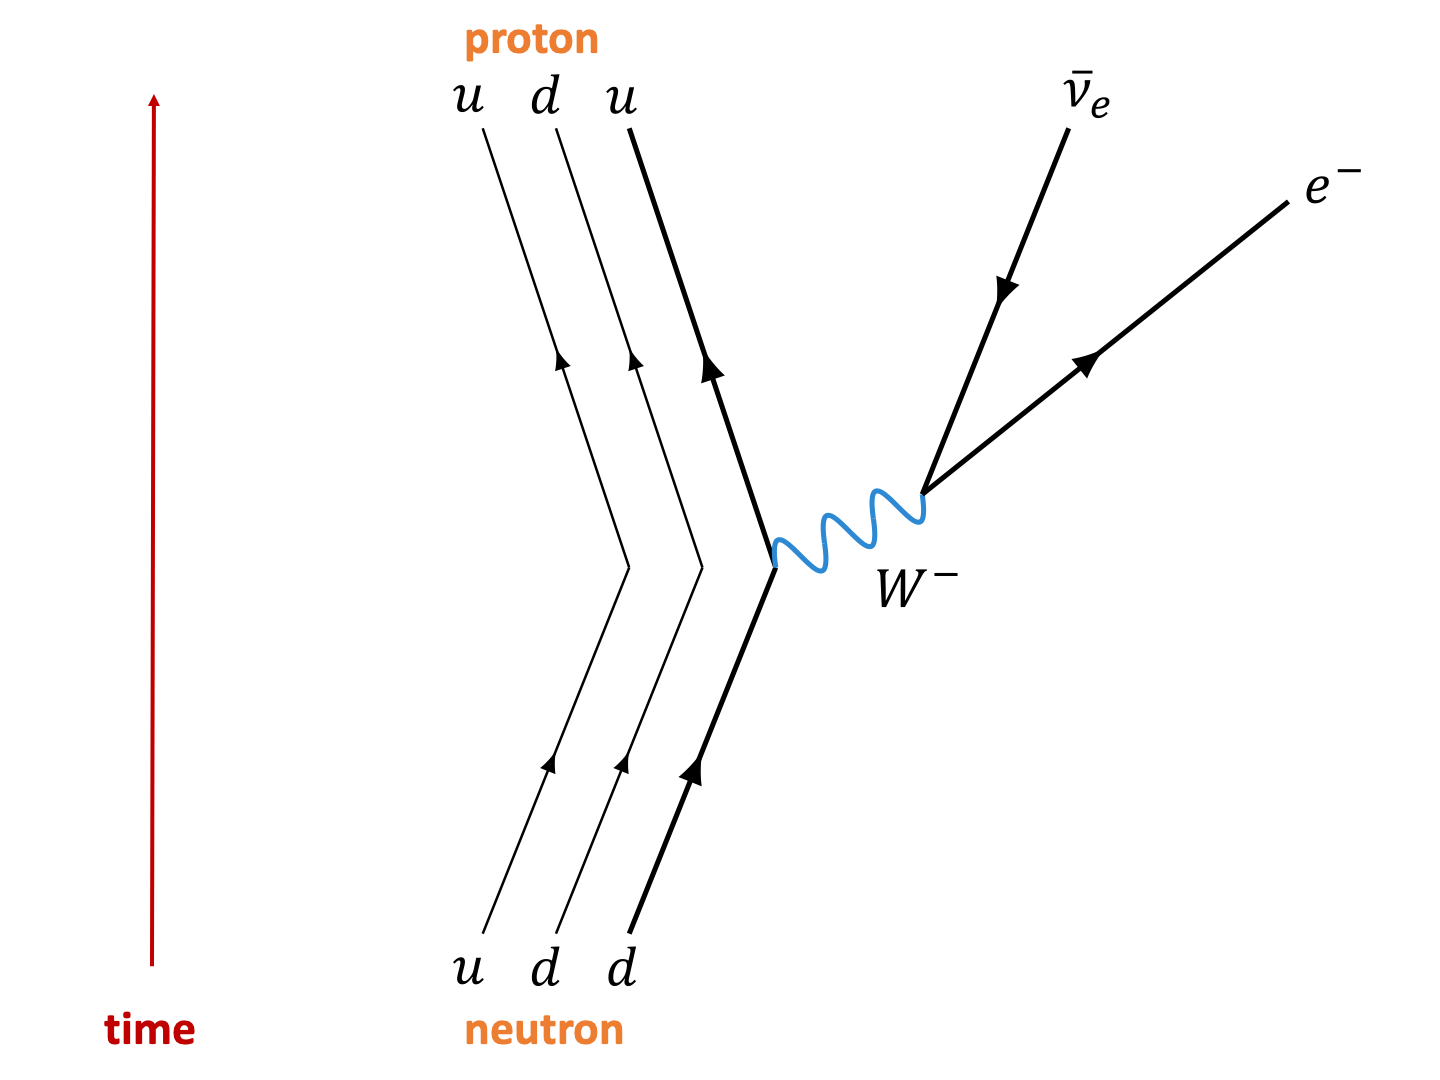
\includegraphics[width=0.6\linewidth]{figures/neutron_decay.png}
	\caption{The Feynman diagram of neutron decay.}
	\label{fig:neutron_decay}
\end{figure}

The discrepancy of knowledge between the proton and the neutron is the last major difference of the nucleons we will discuss here, because it goes directly toward the principle of the BONuS12 Experiment. We know much more about the structure of the proton and momentum distribution of the quarks inside the proton for the reason discussed in the last paragraph. That is, protons can exist outside of nuclei while neutrons soon decay via the weak interaction

\begin{equation}
n \longrightarrow p + e^{-} + \bar{\nu}_{e}
\end{equation}
seen in in Fig. \ref{fig:neutron_decay} as a Feynman diagram. Feynman diagrams were developed by physicist Richard Feynman to display particle interactions that occur in a relatively simplistic manner. Moving from the bottom to the top in the diagram of Fig. \ref{fig:neutron_decay}, we see a down quark within the neutron change states to an up quark mediated by the $W^-$ boson emitting an electron ($e^-$) and electron antineutrino ($\bar{\nu}_{e}$). This decay happens within 15 minutes of a neutron being a free particle. That decay coupled with the fact that the neutron has no electric charge makes isolating neutrons to create a target for scattering experiments extremely difficult. Yet, scattering experiments are the primary means by which physicists study the structure of particles. Therefore, studying the structure of the neutron is inherently made difficult by this lack of free neutron target.

\section{Electron-Scattering Kinematics}
To study the structure and physics of particles, nuclear and particle physicists use scattering experiments. There are two ways of creating a scattering experiment. One way is to accelerate a light particle (an electron, for example) and direct it toward a stationary target, which is the method used at Jefferson Lab in Newport News, Virginia. The other way is to accelerate two particles in opposite directions and then direct the two toward each other, which is the method used at the Large Hadron Collider (LHC) at CERN in Geneva, Switzerland. The physics or kinematics\footnote{The word kinematics refers to the mechanics of the particles without concern for the forces that caused the motion. Essentially, we are not concerned with \textit{how} the particles were accelerated, just that they have a particular energy at the time of collision.} of both scattering experiments is essentially the same. 

When the scattering particle and target collide, some of the momentum and energy of the scattering particle is transfered to that target particle. The way that nuclear and particle physicists express that energy and momentum is in something called its four-momentum. Classical momentum is a vector, which means it has a magnitude and direction. That direction is typically expressed in three dimensions (for the familiar Cartesian coordinate system that would be along the x, y, and z-axis). Therefore a momentum can be expressed as $\mathbf{p}$ = ($p_x$, $p_y$, $p_z$), where $\mathbf{p}$ is the momentum vector bold-faced to indicate that it is a vector. Because in particle physics, the particles travel close to the speed of light, we have to deal with special relativity. For the purposes of this work, special relativity essentially forces us to consider not just three-dimensional space, but four dimensional space-time with different reference frames for any non-accelerating moving objects. This drives us to require there be a four-dimensional space-time momentum $p=(p_0,p_1,p_2,p_3)$, where $p_1=p_x$, $p_2=p_y$, and $p_3=p_z$ in Cartesian coordinates. The new term $p_0$ is equal to $E/c$, where $E$ is the energy of the particle and $c$ is the speed of light.

If we take this four-momentum
\begin{equation}
p_{\mu} = \left( \frac{E}{c}, p_x, p_y, p_z \right),
\end{equation} 
where $\mu$ is just an index indicating a particular particle and square it, we have
\begin{equation}
p^{\mu}p_{\mu} = -\frac{E^2}{c^2} + p^2_x +p^2_y + p^2_z = -\frac{E^2}{c^2} + p^2.
\end{equation}
This quantity should be invariant under a Lorentz transformation (meaning it remains the same no matter the non-accelerating reference frame) and is equal to the Lorentz scalar $-m^2c^2$, which means 
\begin{equation}
\label{eqn:4mom}
-\frac{E^2}{c^2} + p^2 = -m^2c^2.
\end{equation}
Multiplying both sides of Eq. \ref{eqn:4mom} by $-c^2$ and rearranging a little gives us
\begin{equation}
\label{eqn:e_squared}
E^2 = - p^2c^2 + m^2c^4,
\end{equation}
which if we take the square root of both sides results in
\begin{equation}
E=\sqrt{(pc)^2+(mc^2)^2}.
\end{equation}
In the rest frame of the particle ($i.e.$ the frame where the particle is considered to have no momentum, thus $p=0$), this equation reduces to something that should be familiar. That is
\begin{equation}
E=mc^2.
\end{equation}
This rough derivation provides a little insight to the power and purpose of using four-momentum. We will use this notation extensively throughout the rest of this work. 

The other useful notation to understand is called natural units, where $c=\hbar=1$. Under these units, Eq. \ref{eqn:e_squared} becomes
\begin{equation}
E^2 = p^2 + m^2.
\end{equation}
While this offers much in the way of simplicity when working with complex equations, the disadvantage is that we lose information regarding dimensional analysis of the equation. Nevertheless, for the most part, we will use natural units in this work.

Now, consider an electron with four-momentum $k$ scattering off of a nucleon with momentum $p$. The Feynman diagram for such an interaction is in Fig. \ref{fig:feyn_epscatt}, where $k'$ and $p'$ are the final momentum of the scattered electron and nucleon respectively. Here, $q$ is the momentum of the virtual photon\footnote{The term "virtual" here may be misleading. It does not imply that the photon does not really exist. It refers to the short-lived exchange of the electromagnetic force.} (typically denoted by $\gamma^{*}$ ) that mediates the interaction. That virtual photon momentum is defined as $q=k'-k$, which implies that it is the momentum lost by the scattered electron.

\begin{figure}[h!]
	\centering
	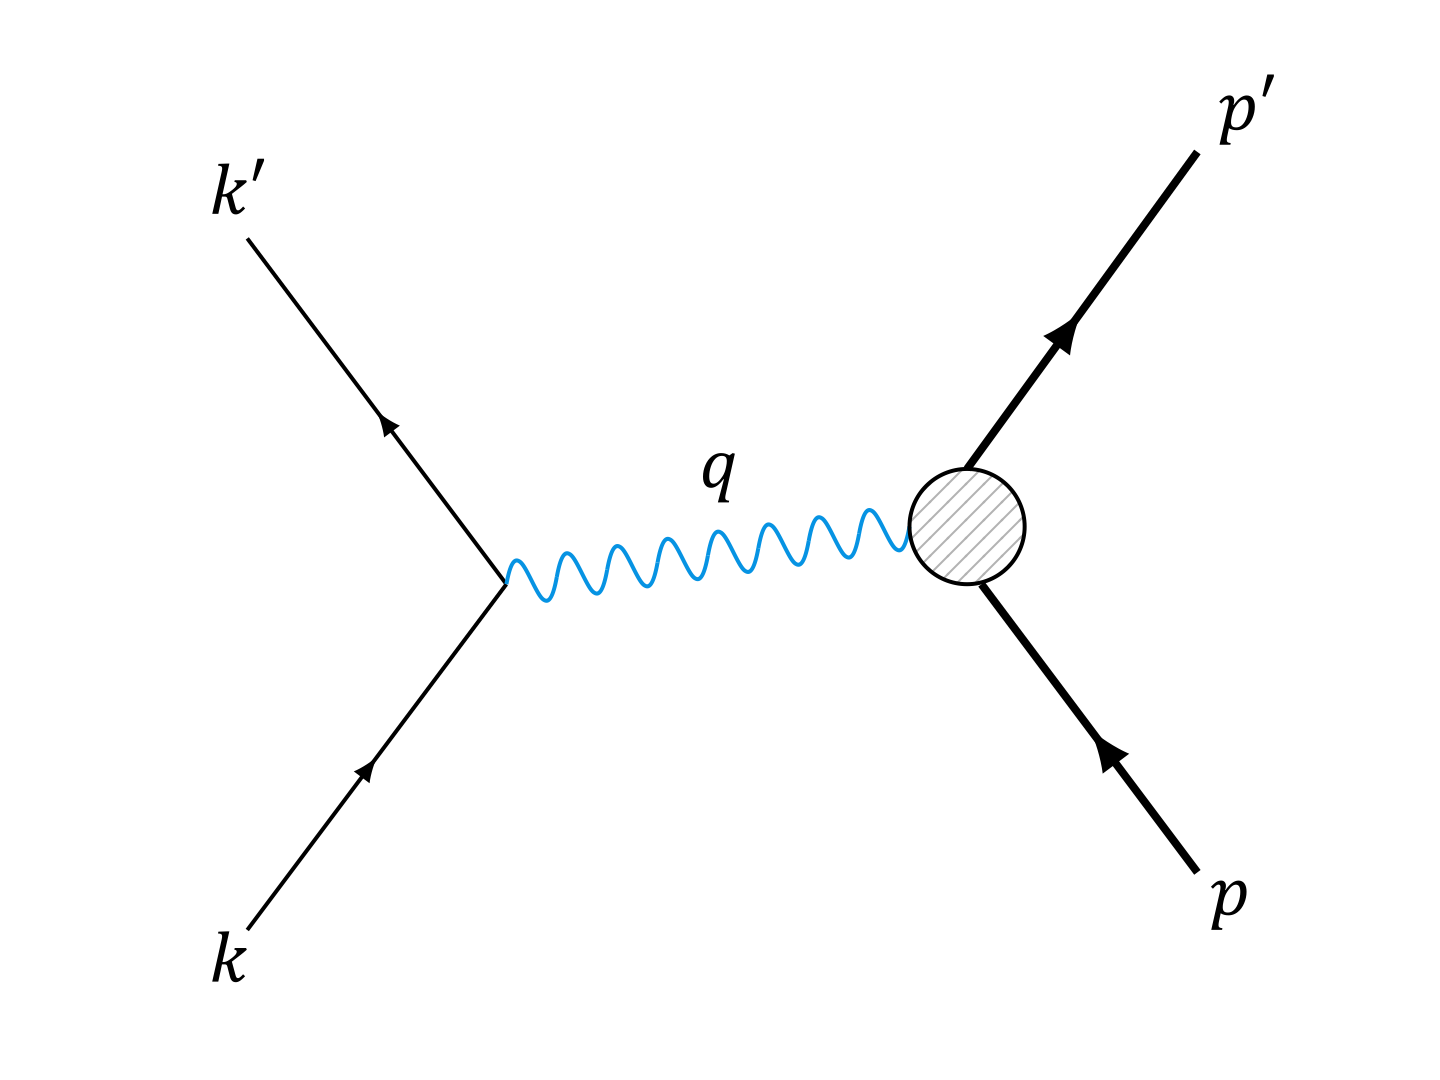
\includegraphics[width=0.6\linewidth]{figures/feyn_epscatt.png}
	\caption{Feynman diagram of an electron scattering from a proton.}
	\label{fig:feyn_epscatt}
\end{figure}

There are some other important quantities to consider for electron scattering. The first is the square of that four-momentum transfer
\begin{equation}
q^2 = (k' - k)^2 = 2m_e^2 - 2(EE' - |\mathbf{p}||\mathbf{p}'| \cos \theta),
\end{equation}
where $m_e$ is the mass of the electron, $E$ is the energy of the incident electron, $E'$ is the energy of the scattered electron, $|\mathbf{p}|$ is the magnitude of the three-momentum of the incident nucleon, $|\mathbf{p}'|$ is the magnitude of the incident nucleon's three-momentum, and $\theta$ is the scattering angle of the electron. When we use the trigonometric identity $1-\cos \theta = 2 \sin^2 \tfrac{\theta}{2}$ and take the electron mass to be zero, we get
\begin{equation}
q^2 \approx -4EE'\sin^2\tfrac{\theta}{2}.
\end{equation}
As a convention to make the quantity positive, we use $Q^2 = -q^2$, which will be used throughout the rest of this work. Another variable we need to analyze these electron scattering kinematics is the variable $\nu$, which is the energy transfer of the electron to the nucleon via $\gamma^*$ ($i.e.$ the virtual photon) and is defined by
\begin{equation}
\nu = \frac{p \cdot q}{M}.
\end{equation}
Here, $p$ is the four-momentum of the incident nucleon, $q$ is the four-momentum of the incident electron and $M$ is the nucleon mass. In the laboratory frame, the nucleon is at rest ($i.e.$ $p=(M,\mathbf{0})$)\footnote{Just like other three-dimensional vectors, when bolded, $\mathbf{0}$ represents (0,0,0).}, and $q=(E-E',\mathbf{q})$, so the energy transfered by the virtual photon to the nucleon in the laboratory frame would be
\begin{equation}
\nu  = E-E'.
\end{equation}

\begin{figure}[h!]
	\centering
	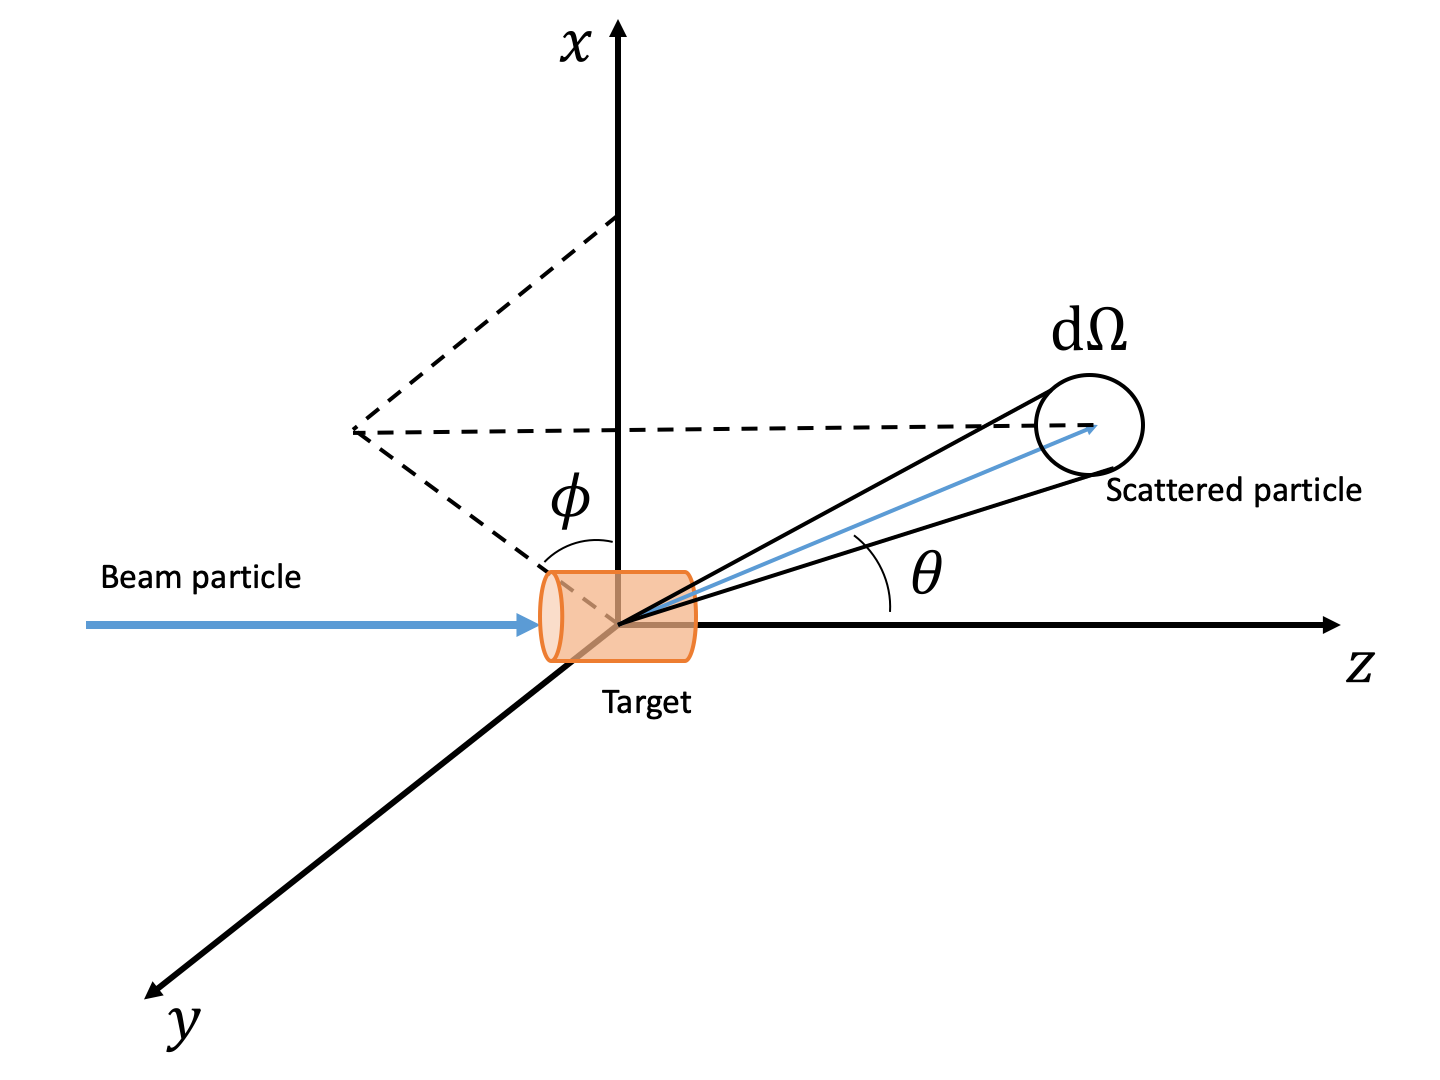
\includegraphics[width=0.6\linewidth]{figures/diff_xsec.png}
	\caption{Scattering process on a quasi-static Differential cross section.}
	\label{fig:diff_xsec}
\end{figure}

Whenever we deal with collisions of particles, there is a probability associated with the reaction between that projectile and target depicted in Fig. \ref{fig:diff_xsec}. That probability is called the \textit{cross section} and with it often comes a wealth of knowledge about the dynamics of the interaction itself. In many reactions we deal with what is known as the \textit{differential} cross section, which offers a more realistic insight to only a fraction of reactions. This differential cross section is ratio of the number of particles per unit time scattered into a bit of the solid angle $\mathrm{d}\Omega$. Mathematically, the cross section of a spinless particle scattered from a static point charge the differential cross section can be written as 
\begin{equation}
\label{eqn:rutherford}
\frac{\mathrm{d}\sigma}{\mathrm{d}\Omega} = \frac{\alpha^2}{4E^2\sin^4 \frac{\theta}{2}},
\end{equation}
where $\alpha$ is known as the fine-structure constant equal to $e^2/4\pi \approx 1/137$, $E$ is the energy of the incident electron, and $\theta$ is the scattering angle of the electron in the laboratory frame. Eq. \ref{eqn:rutherford} is known as the Rutherford Formula and is the simplest theoretical scattering case. If we include the electron spin, we get
\begin{equation}
\label{eqn:mott}
\frac{\mathrm{d}\sigma}{\mathrm{d}\Omega} = \frac{\alpha^2 \cos^2 \frac{\theta}{2}}{4E^2\sin^4 \frac{\theta}{2}},
\end{equation}
which is known at the \textit{Mott} cross section (we will from now on denote this particular cross section by $\left( \tfrac{\mathrm{d}\sigma}{\mathrm{d}\Omega} \right)_{\mathrm{Mott}}$). If we next introduce the mass of the point-like target $M$, that target particle will recoil, and so we get a scattered electron energy of 
\begin{equation}
E' = \frac{E}{1+\frac{2E}{M}\sin^2 \frac{\theta}{2}},
\end{equation}
modifying the Mott cross section to
\begin{equation}
\frac{\mathrm{d}\sigma}{\mathrm{d}\Omega} = \left( \frac{\mathrm{d}\sigma}{\mathrm{d}\Omega} \right)_{\mathrm{Mott}} \cdot \frac{E'}{E} \left[ 1-\frac{q^2}{2M^2}\tan^2 \frac{\theta}{2} \right] = \frac{\alpha^2 \cos^2 \frac{\theta}{2}}{4E^2\sin^4 \frac{\theta}{2}} \cdot \frac{E'}{E} \left[ 1-\frac{q^2}{2M^2}\tan^2 \frac{\theta}{2} \right].
\end{equation}
As that target mass $M$ increases, this equation reduces to the Mott cross section. 

We are beginning to approach a more realistic mathematical description of scattering, so we must discuss the various types that exist. In Fig. \ref{fig:feyn_epscatt} if both particles remain intact after the collision, it is called \textit{elastic scattering}. Like pool balls, they essentially bounce off each other, of course through the exchange of that virtual photon. When the amount of energy transfer increases ($i.e.$ when $q$ increases), different types of scattering arise. We need to understand these types of scattering in more depth to understand the BONuS12 Experiment.
\newpage
\section{Elastic Scattering}
When the momentum transfer, or more specifically $Q^2$, is low, there is a higher probability that the lepton (at JLab, that lepton is an electron) essentially bounces off of the target particle (typically a nucleon) in what is known as elastic scattering. Whatever momentum is transferred does not force the nucleon into excited states (called resonances) or break it apart entirely (deep inelastic scattering). In a situation like Fig. \ref{fig:feyn_epscatt} when scattering elastically
\begin{equation}
k+p \longrightarrow k' + p'
\end{equation}
or
\begin{equation}
k + p = k' + p'
\end{equation}
indicating the conservation of energy and momentum. Here $k$ and $p$ are the incident electron and nucleon four-momenta respectively, and $k'$ and $p'$ are the scattered electron and nucleon respectively. In this elastic case,
\begin{equation}
(k+q)^2 = p^2 = M_N^2,
\end{equation}
where $M_N$ is the mass of the nucleon. 

Because these particles are not point-like, we cannot simply use the Mott Equation (Eq. \ref{eqn:mott}) to calculate the cross section of this elastic-scattering process. If we scatter electrons from some particle with a charge distribution $\rho(r)$ (here $\rho(r)$ is the charge distribution which is dependent on the distance away $r$ from the charge source), like a proton, the scattering amplitude is modified by something called a form factor
\begin{equation}
\label{eqn:ff}
F(q^2) = \int d^3r \; e^{i\mathbf{q} \cdot \mathbf{r}} \; \rho(r).
\end{equation}
This particular form factor in Eq. \ref{eqn:ff} is an integral over volume of that charge distribution times the plane-wave of the particle, and is just the Fourier Transform of the charge density. As the name suggests this form factor provides insight into the composite structure of that particle. When this form factor is squared, it serves as a multiplier to the the Mott cross section, giving us an expression for elastic scattering
\begin{equation}
\frac{\mathrm{d}\sigma}{\mathrm{d}\Omega} = \left( \frac{\mathrm{d}\sigma}{\mathrm{d}\Omega} \right)_{\mathrm{Mott}} [F(q^2)]^2,
\end{equation}
where the Mott cross section found in Eq. \ref{eqn:mott} is elastic electron scattering off a point-like Dirac particle\footnote{A Dirac particle refers to a particle whose wave-function $\psi$ obeys the Dirac equation \\ $(i\slashed{\partial} - m)\psi = 0$. The ``slashed" notation is used to indicate $\slashed{\partial} \overset{\mathrm{def}}{=}\gamma^{\mu} \partial_{\mu}$, where $\gamma^{\mu}$ are the set of Pauli matrices.}. This gives us a useful description of elastic electron-proton scattering.

The last thing to do regarding the elastic scattering cross section is to expand the expression into the kinematic variables we can measure. We accomplish this by defining a scattering probability amplitude $\mathcal{M}$ such that in the lab frame
\begin{equation}
\frac{d\sigma}{d\Omega} = \frac{1}{64\pi^2} \left( \frac{1}{M_p + 2E \sin^2 \frac{\theta}{2}} \right)^2 |\mathcal{M}_{fi}|^2,
\end{equation} 
where we neglect the small electron mass, $M_p$ is the mass of the proton, $E$ is the incident electron energy, and $\theta$ is the scattering angle of the electron in the lab frame. The term $|\mathcal{M}_{fi}|^2$ is shorthand for
\begin{equation}
|\mathcal{M}_{fi}|^2 = |\bra{f} \mathcal{M} \ket{i}|^2,
\end{equation}
which means that we find the modulus squared expectation value of the observable $\mathcal{M}$ for the initial and final states. If the polarizations are not observed, this must be averaged over initial spin states of the modulus squared of the scattering amplitudes and the summed over the final spin states of $|\mathcal{M}|^2$. Mathematically, using $s$ and $S$ for initial spin states of the electron and proton respectively and $s'$ and $S'$ for final spin states, it can be expressed as
\begin{equation}
|\mathcal{M}_{fi}|^2 = \frac{1}{2} \frac{1}{2} \sum_{s,S} \sum_{s',S'} |\mathcal{M}|^2,
\end{equation}
where $\mathcal{M}$ is the scattering probability amplitude. 

\begin{figure}[h!]
	\centering
	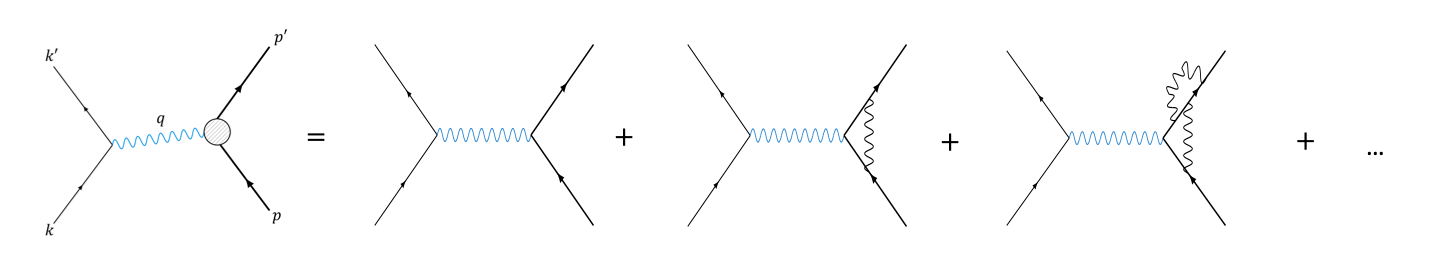
\includegraphics[width=\linewidth]{figures/feyn_sum.png}
	\caption{The contributions of higher order diagrams.}
	\label{fig:feyn_sum}
\end{figure}

The scattering probability amplitude cannot be known exactly because of the processes beyond the first order (tree level) that could occur in Fig. \ref{fig:feyn_epscatt} at the proton-$\gamma^{*}$ vertex blob (these contributions can be seen in Fig. \ref{fig:feyn_sum}). However, we can handle the mathematical description of these processes by expressing the scattering probability amplitude matrix it in terms of the leptonic and hadronic tensors, we have
\begin{equation}
\label{eqn:el_M2}
|\mathcal{M}|^2 = \frac{e^4}{Q^4} \ell_{\mu\nu} W^{\mu \nu}.
\end{equation}
The leptonic tensor $\ell_{\mu\nu}$ is associated with the coupling of the virtual photon to the electron (more generally the coupling of the exchange boson to the lepton), and for unpolarized scattering can be expressed as
\begin{equation}
\label{eqn:lep_tens}
\ell_{\mu\nu} = \bar{u}(k',s')\gamma^{\mu}u(k,s) \bar{u}(k,s) \gamma^{\nu} u(k',s').
\end{equation}
The term $u(k)$ is the Dirac spinor. For the electron (a spin-$1/2$ fermion), there are two spin states ($i.e.$ up or down) so there are two associated spinors that could exist here
\begin{equation}
u_{\uparrow}(k) = \left( \begin{array}{c} 1 \\ 0 \\ \frac{k_z}{E+m} \\ \frac{k_x+ik_y}{E+m} \end{array} \right) \; \; \mathrm{and} \; \;
u_{\downarrow}(k) = \left( \begin{array}{c} 0 \\ 1 \\ \frac{k_x-ik_y}{E+m} \\ \frac{-k_z}{E+m} \end{array} \right).
\end{equation}
In Eq. \ref{eqn:lep_tens}, $\gamma^{\mu}$ are the gamma matrices. When summed and averaged over spins, the leptonic tensor becomes
\begin{eqnarray}
\nonumber
\ell_{\mu\nu} &=& \mathrm{Tr} \left[ \frac{\slashed{k}'+m}{2m} \gamma^{\mu} \frac{\slashed{k}+m}{2m} \gamma^{\nu} \right] \\
\nonumber
&=& \frac{1}{m^2} \mathrm{Tr} (\slashed{k}'\gamma^{\mu}\slashed{k}\gamma^{\nu} + m^2\gamma^{\mu}\gamma^{\nu}) \\
&=& 2 (k'^{\mu}k^{\nu} + k^{\mu}k'^{\nu} - g^{\mu\nu}k' \cdot k).
\end{eqnarray}
Thus far we have from Eq. \ref{eqn:el_M2}
\begin{equation}
|\mathcal{M}|^2 = \frac{e^4}{Q^4} 2 (k'^{\mu}k^{\nu} + k^{\mu}k'^{\nu} - g^{\mu\nu}k' \cdot k) W^{\mu \nu},
\end{equation}
where $g{\mu\nu}$ is the metric tensor.

We must now take a look at the hadronic tensor $W^{\mu\nu}$, which is more complicated because we must take into account for the proton's structure. In fact, the hadronic tensor cannot be known exactly. It can, however, be expanded to the second order as
\begin{equation}
W^{\mu\nu} = \bra{p}J^{\nu}\ket{p'}\bra{p'}J^{\mu}\ket{p},
\end{equation}
which depends on the $J^{\mu}$ current matrix elements. That current between two nucleon states
\begin{equation}
\bra{p}J^{\mu}(0)\ket{p'} = \bar{U}(p')\left[ F_1(Q^2)\gamma^{\mu}+F_2(Q^2)\frac{i\sigma^{\mu\nu}}{2M_N} \right]U(p)
\end{equation}
gives rise to two form factors, $F_1(Q^2)$ which is called the Dirac form factor and $F_2(Q^2)$ called the Pauli form factor. Here $\sigma^{\mu\nu}=\tfrac{i}{2}[\gamma^{\mu},\gamma^{\nu}]$ and we denote the difference between the lower-case $u(k,s)$ electron spinors from Eq. \ref{eqn:lep_tens} and upper-case $U(p)$ nucleon spinors. If we introduce the more physically interesting Sach's electric and magnetic form factors respectively
\begin{equation}
\nonumber
G_E(Q^2) = F_1(Q^2) + \frac{Q^2}{4M_N^2} F_2(Q^2)
\end{equation}
\begin{equation}
\nonumber
G_M(Q^2) = F_1(Q^2) + F_2(Q^2),
\end{equation}
then the hadronic tensor can be written as
\begin{eqnarray}
\nonumber
W^{\mu\nu} &=& 2(p'^{\mu}p^{\nu} + p'^{\nu}p^{\mu} - g^{\mu\nu}(pp'-M_N^2))G_M^2 \\
\nonumber
&&- 2F_2G_M(p+p')^{\mu}(p+p')^{\nu}+F_2^2\frac{M_N^2+p \cdot p'}{2M_N^2}(p+p')^{\mu}(p+p')^{\nu} \\
\nonumber
&=& (-q^{\mu}q^{\nu}+g^{\mu\nu}q^2)G_M^2+(p+p')^{\mu}(p+p')^{\nu}\frac{G_E^2+\tau G_M^2}{1+\tau} \\
&=& g^{\mu\nu}q^2G_M^2+4p^{\mu}p^{\nu}\frac{G_E^2+\tau G_M^2}{1+\tau} + ...,
\end{eqnarray} 
where we define $\tau = Q^2/4M_N^2$ to simplify the expression. Because of current conservation, the terms contain factors of $q^{\mu}$ are omitted with the ellipses, since they do not contribute to the cross section.

Substituting our expressions for the leptonic and hadronic tensors for elastic scattering in the lab frame and contracting them, we arrive at
\begin{equation}
\label{eqn:el_cs}
\frac{d\sigma}{d\Omega} = \left( \frac{d\sigma}{d\Omega} \right)_{\mathrm{Mott}} f_{\mathrm{rec}} \left[ \frac{G_E^2(Q^2) + \tau G_M^2(Q^2)}{1+\tau} + 2\tau G_M^2 \tan \frac{\theta}{2} \right],
\end{equation}
where $\left( \tfrac{\mathrm{d}\sigma}{\mathrm{d}\Omega} \right)_{\mathrm{Mott}}$ comes from Eq.\ref{eqn:mott} ($i.e.$ the Mott cross section) and $f_{\mathrm{rec}}$ is the recoil factor equal here to $E'/E$. As $Q^2$ gets very high, $\tau$ increases and magnetic form factor $G_M(Q^2)$ dominates. This gives a more physical description of the elastic scattering cross section in terms of kinematic variables that can be measured through scattering experiments.

One more kinematic variable that needs to be introduced offers insight into cases when scattering enters into inelastic regimes. The invariant mass squared $W^2$ (not to be confused with the hadronic tensor $W^{\mu\nu}$) of the photon-nucleon system, is defined mathematically as 
\begin{equation}
W^2 = (q+p)^2 =M_N^2 + 2M_N\nu - Q^2,
\end{equation}
where $\nu = E-E'$ is the energy transfered from the electron to the nucleon via virtual photon ($\gamma^*$). In the elastic scattering case , $W^2 = M_N^2$, because $Q^2$ and thus $\nu$ tend to be small ($i.e.$ $E << M_N$). As $Q^2$ increases, instead of simply bouncing off of the nucleon, the energy transfered to the nucleon begins changing the state of the quarks within the nucleon. 

\section{Resonance Region}
Changing the state of a quark within the nucleon results in excited states of that nucleon, called \textit{resonances}. The region where resonances occur is $M_N^2 < W^2 < 4 \; \mathrm{GeV}^2$, and is called the \textit{resonance region}. There are 6 families of resonances that depend on the characteristics of the resonant particles. Particles containing only $u$ and $d$ quarks whose isospin $I= \tfrac{1}{2}$ are denoted by $N$. The $\Delta$ family of resonances also have only $u$ and $d$ quarks, but have $\tfrac{3}{2}$ isospin. When $I=0$ and the particle contains $u$, $d$ and one $c$, $s$, or $b$ quark, it is called a $\Lambda$ resonance. The $\Sigma$ resonance also has $u$, $d$ plus one $c$, $s$, or $b$ quark, but with $I=1$. When only one $u$ or $d$ quark exists with two $c$, $s$, or $b$ quarks with $I=\tfrac{1}{2}$, it is a $\Xi$ resonance. Finally, when $I=0$ and only $c$, $s$, or $b$ quarks are present, it is known as an $\Omega$ resonance.

Unlike the ground state of nucleons, these excited states are extremely short lived (on the order of $10^{-23}$ seconds). After their short life, these resonances decay into more stable hadrons. Detection of the these hadrons is what provides proof of the existence of resonant states. For example, a common resonance $\Delta^0(1232)$, which is the lowest lying resonance with a mass of $1.232$ GeV, predominately decays via the strong interaction into a pion ($\pi^0$) and a neutron ($n$). The entire interaction begins at the first step of creating an excited state
\begin{equation}
p+e^- \longrightarrow \Delta^0
\end{equation}
then decays into
\begin{equation}
\Delta^0 \longrightarrow \pi^0 + n.
\end{equation}
However, because these resonances are so short-lived, it is convention to express the entire interaction as
\begin{equation}
\label{eqn:delta_res}
p+e^- \longrightarrow \pi^0 + n.
\end{equation}
One reason for this convention is that there are many resonances that can produce the same end particles ($i.e.$ $\pi^0$ and $n$ in our example). Knowing exactly what resonance produced those end particles can be difficult. In the example of Eq. \ref{eqn:delta_res}, the $\Delta^0$ has the same quark makeup as the neutron ($i.e.$ $udd$), but is much heavier. Measuring the invariant mass of the resulting particles is one of the few ways to understand what resonance occurred. 

Similar to elastic scattering, interactions with resonances can be described using form factors. The analogous cross section is
\begin{equation}
\frac{d\sigma}{d\Omega} = \left( \frac{d\sigma}{d\Omega} \right)_{\mathrm{Mott}} f_{\mathrm{rec}} \left( \frac{|G_E|^2+\tau^*|G_T|^2}{1+\tau^*} + 2\tau^* |G_T|^2 \tan^2 \frac{\theta}{2} \right) R(W),
\end{equation}
where $f_{\mathrm{rec}}$ is the recoil factor of the proton, $\tau^*$ is the analogous kinematic quantity of $\tau$ from elastic scattering, $G_E$ and $G_T$ are the resonance longitudinal and transverse form-factors respectively, and $R(W)$ is called the resonance line shape. In inelastic scattering of resonances
\begin{equation}
f_{\mathrm{rec}} = \frac{E'}{E} \left[ \frac{1}{1-\frac{(W_R^2 - M_N^2)}{2M_NE}} \right],
\end{equation}
\begin{equation}
\tau^* |G_T|^2 = \frac{1}{2}(|G_+|^2 + |G_-|^2),
\end{equation}
and
\begin{equation}
R(W) = \frac{2\pi^{-1}W_R M_N \Gamma_R}{(W^2-W_R^2)^2 + W_R^2 \Gamma_R^2}.
\end{equation}
The quantities $W_R$ and $\Gamma_R$ refer to the resonance mass and width respectively. If the resonance width is small enough ($i.e.$ when $W_R=M_N$ and $W_R \Gamma_R \rightarrow 0$), $R(W)$ becomes a $\delta$-function and the resonance cross section reduces to that of an elastic cross section. 

At low $Q^2$, we can describe interactions by constituent quarks models. At high $Q^2$ we enter a region best described with perturbative quantum chromodynamics (pQCD). We will discuss more about pQCD in a later section. The resonant region is an important bridge between these two regimes. Determining resonance form factors allows us to describe the resonance transition the same way elastic form factors describes elastic interactions.

\section{Deep Inelastic Scattering}
Once the energy transfered to the nucleon ($Q^2$) becomes large enough, the probability of creating excited (resonance) states decreases and there becomes a higher probability of the virtual photon ``elastically" scattering off a quark inside the nucleon. This is known as \textit{deep} inelastic scattering. This happens around when $W > 2$ MeV and $Q^2 > 1$ $\mathrm{GeV}^2$ in an area known as the \textit{continuum}. In this regime we can probe the inner structure of the nucleon. 

\begin{figure}[h!]
	\centering
	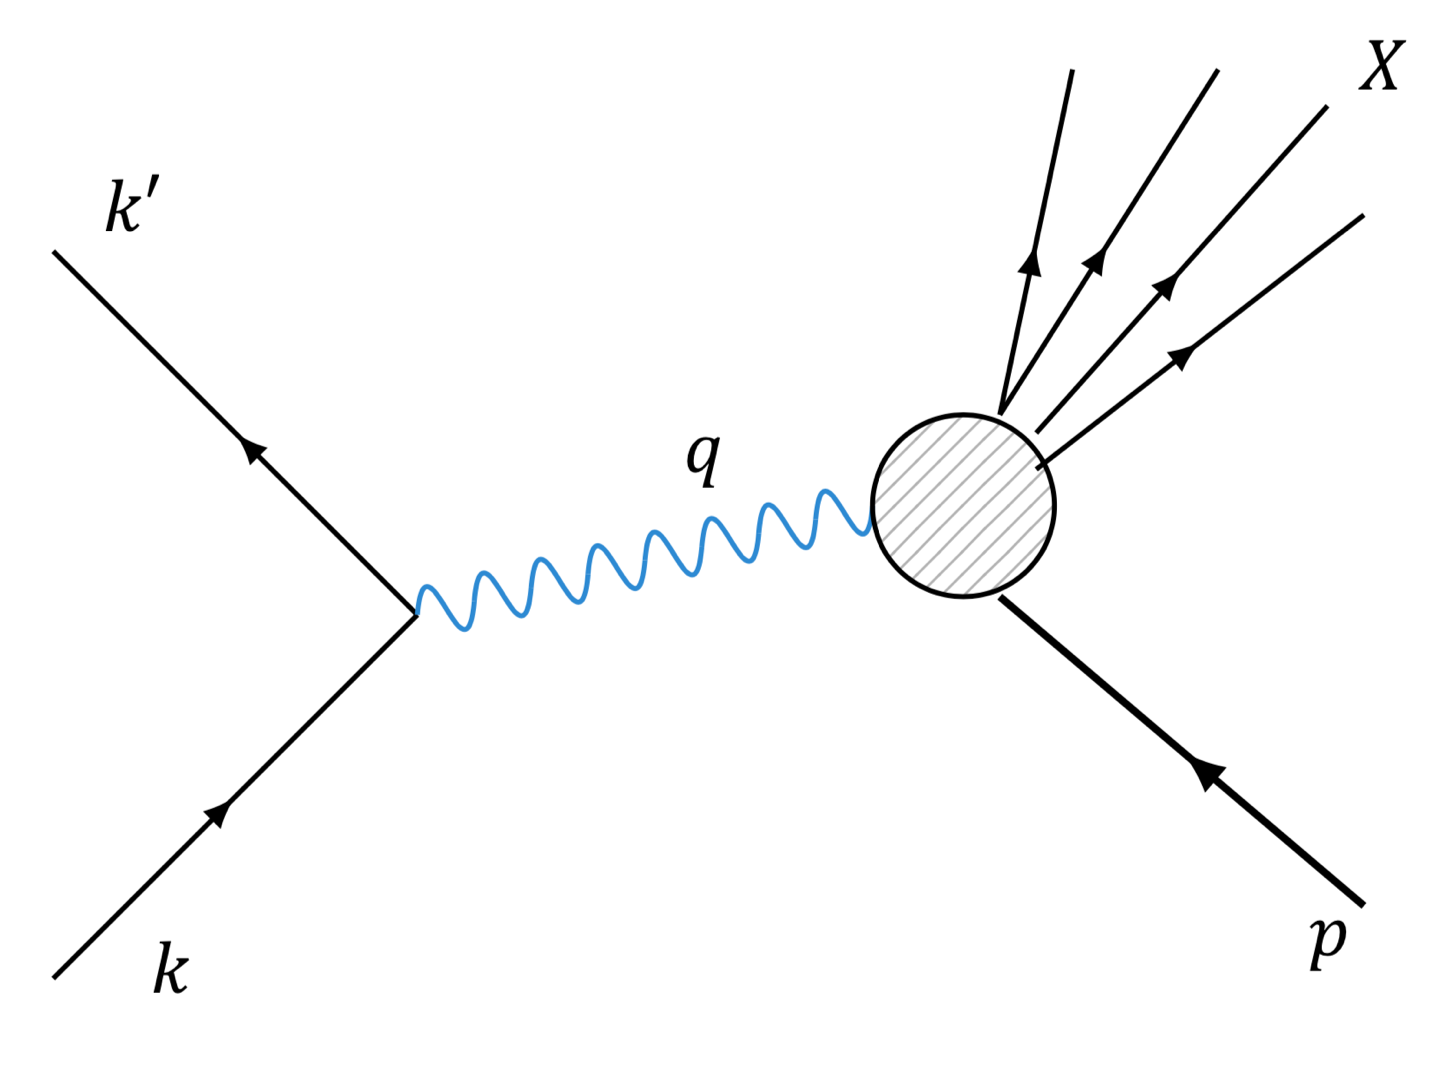
\includegraphics[width=0.6\linewidth]{figures/feyn_inelscatt.png}
	\caption{Feynman diagram of an inelastic electron scattering from a proton.}
	\label{fig:feyn_inelscatt}
\end{figure}

However, because the energy transfer is so high, the proton often breaks apart in the interaction
\begin{equation}
ep \longrightarrow eX,
\end{equation}
where $X$ denotes all possible particles that might emerge from the proton-electron collision. The Feynman diagram also must be altered from Fig. \ref{fig:feyn_epscatt} to Fig. \ref{fig:feyn_inelscatt}, where $X$ again represents all possible emerging particles. The other change from elastic and inelastic resonance-region scattering is to the cross section. This deep-inelastic scattering cross section can be written as
\begin{equation}
\frac{d\sigma}{dE'\Omega} = \frac{4\alpha^2E'^2}{q^4} W_2(\nu,Q^2)\cos^2\frac{\theta}{2} +2W_1(\nu,Q^2) \sin^2 \frac{\theta}{2},
\end{equation}
where $W_1$ and $W_2$ are called inelastic structure functions. These structure functions are the analogs to the form factors in Eq. \ref{eqn:el_cs} for elastic scattering. There is much more to discuss about deep-inelastic scattering, but first we must discuss how to treat scattering off of quarks (or more broadly, partons) within a nucleon with an approach called \textit{scaling}.

\section{Partons and Bjorken-Scaling}
The way we probe inside nucleons is with the exchange of small wavelength (large $Q^2$) virtual photons, which break apart the proton. This can be handled using the inelastic structure functions $W_1$ and $W_2$, which are functions of the energy lost by the electron due to proton recoil ($i.e.$ $\nu$) and the negative four-momentum squared of the virtual photon ($i.e.$ $Q^2$). When the virtual photon has a small enough wavelength (large enough $Q^2$), the nucleon that was once described by Eq. \ref{eqn:el_cs} starts to look more like a free Dirac particle described by
\begin{equation}
\label{eqn:quark_scatt}
\frac{d\sigma}{dE'd\Omega} = \frac{4 \alpha^2 e_q^2 E'^2}{q^4} \left( \cos^2 \frac{\theta}{2} - \frac{q^2}{2m^2}\sin^2 \frac{\theta}{2} \right) \delta \left( \nu + \frac{q^2}{2m} \right).
\end{equation} 
Remarkably, this is the equation for an electron elastic scattering from a structureless particle. Here $e_q$ is the fractional charge of that structureless particle and $m$ is that particle's mass. This particle inside the nucleon was eventually called a quark.

\begin{figure}[h!]
	\centering
	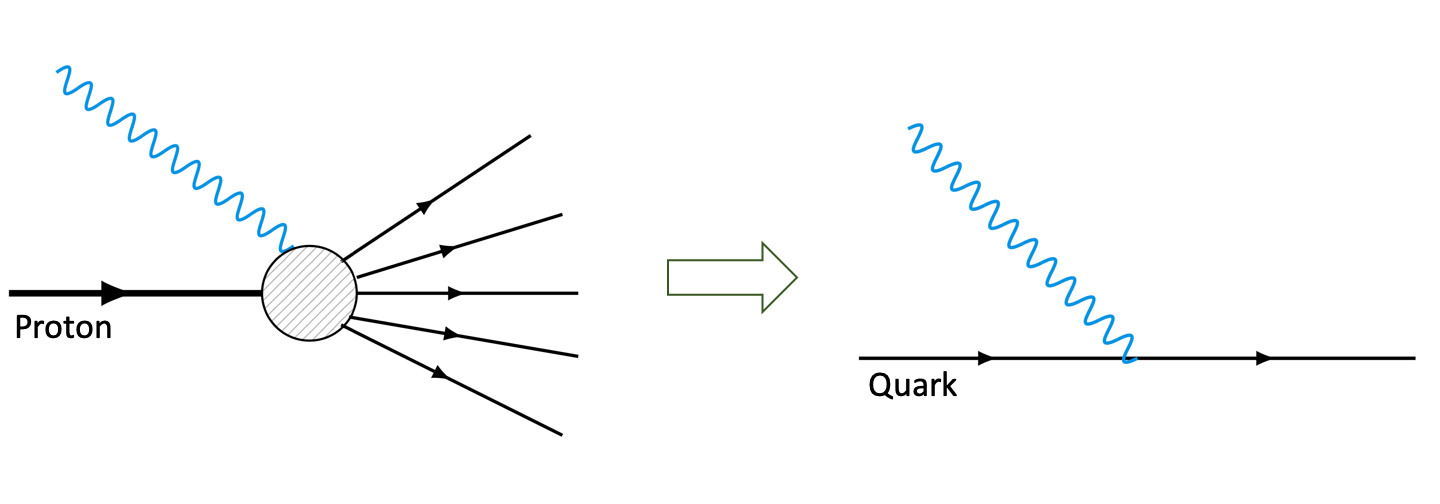
\includegraphics[width=0.9\linewidth]{figures/inel_to_dis.png}
	\caption{The transition from inelastic scattering to deep inelastic scattering of a virtual photon and the quark within a nucleon.}
	\label{fig:feyn_inel_to_dis}
\end{figure}

In this case, where the photon elastically scatters off of a quark within the nucleon described by Eq. \ref{eqn:quark_scatt}, the nucleon structure functions become
\begin{equation}
\label{eqn:dis_sf_1}
2W_1^{\mathrm{point}} = \frac{Q^2}{2m^2} \delta \left( \nu - \frac{Q^2}{2m} \right)
\end{equation}
and
\begin{equation}
\label{eqn:dis_sf_2}
W_2^{\mathrm{point}} = \delta \left( \nu - \frac{Q^2}{2m} \right).
\end{equation}
Here and thus in Eq. \ref{eqn:quark_scatt} there exists the delta function that conserves energy in the interaction. Fig. \ref{fig:feyn_inel_to_dis} shows the resulting diagram when we take the right side of Fig. \ref{fig:feyn_inelscatt} (the left side of Fig. \ref{fig:feyn_inel_to_dis}) and begin to probe a single quark inside the nucleon (the right side of Fig. \ref{fig:feyn_inel_to_dis}). This reduction is representative of the electron elastically scattering off a quark in the nucleon.

If we take Eq. \ref{eqn:dis_sf_1} and \ref{eqn:dis_sf_2}, using the identity $\delta(x/a) = a\delta(x)$, we can write
\begin{equation}
\nonumber
2mW_1^{\mathrm{point}}(\nu,Q^2) = \frac{Q^2}{2m\nu} \delta \left( 1- \frac{Q^2}{2m\nu} \right)
\end{equation}
\begin{equation}
\nu W_2^{\mathrm{point}}(\nu,Q^2) = \delta \left( 1- \frac{Q^2}{2m\nu} \right).
\end{equation}
These equations for the structure functions are now dimensionless and depend on only the ratio $Q^2/2m\nu$, which is both important and useful. That usefulness is as follows: when $Q^2$ is high enough, the virtual photon begins to elastically scatter off of structureless (point) particles  within the nucleon and can be described using the dimensionless structure functions
\begin{equation}
\nonumber
MW_1(\nu,Q^2) \xrightarrow[\text{large $Q^2$}]{} F_1(x_B)
\end{equation}
\begin{equation}
\nu W_2(\nu,Q^2) \xrightarrow[\text{large $Q^2$}]{} F_2(x_B).
\end{equation}
Here $x_B$ is introduced as the Bjorken-$x$ scaling variable defined as
\begin{equation}
x_B = \frac{Q^2}{2M\nu},
\end{equation}
which describes the momentum fraction of a quark or gluon within a nucleon. Up to this point, we have only been discussing interactions between the virtual photon and the quarks within the nucleon, but that virtual photon can also interact with gluons that exits in the nucleon. Collectively, these quarks and gluons in the nucleon are known as partons. The Bjorken-$x$ scaling variable can describe the momentum fraction of any parton within a nucleon.

The relationship between the structure functions $F_1(x_B)$ and $F_2(x_B)$ is
\begin{equation}
2x_B F_1(x_B) = F_2(x_B) = \sum_i e_i^2 f_i (x_B), 
\end{equation} 
where in the right side of this expression we have a sum over partons (the parton index is $i$) of the square of that parton's charge squared ($e_i^2$) times $f_i(x_B)$ known at the parton distribution function. The parton distribution function (or PDF) 
\begin{equation}
f_i(x_B) = \frac{dP_i}{dx_B}
\end{equation}
describes the probability $P_i$ that a struck parton $i$ carries a fraction ($x_B$) of the nucleon's momentum.

Because $F_1(x_B)$ can be calculated using $F_2(x_B)$ using the Callan-Gross relation $2x_B F_1(x_B) = F_2(x_B)$, the $F_2$ structure function is the more important term here to examine experimentally and is of interest in the BONuS12 Experiment. For deep-inelastic electron-proton scattering, the $F_2^p(x_B)$ structure function is
\begin{eqnarray}
\label{eqn:F_p}
\frac{1}{x_B} F_2^p(x_B) &=& \left( \frac{2}{3} \right)^2 [u^p(x_B)+\bar{u}^p(x_B)] + \left( \frac{1}{3} \right)^2 [d^p(x_B)+\bar{d}^p(x_B)] \\
&& + \left( \frac{1}{3} \right)^2 [s^p(x_B)+\bar{s}^p(x_B)],
\end{eqnarray}
where $p$ superscript denotes that we are dealing with the proton structure, and the PDF $f_i(x_B)$ is replaced with the first letter of the quark name ($e.g.$ the up quark and antiquark PDF's are denoted as $u^p(x_B)$ and $\bar{u}^p(x_B)$ respectively). The contributions of quarks heavier than the strange quark have been assumed to be negligible here. The neutron structure function $F-2^n(x)$, where we have dropped the $B$ in $x_B$, is
\begin{eqnarray}
\label{eqn:F_n}
\frac{1}{x} F_2^n(x) &=& \left( \frac{2}{3} \right)^2 [u^n(x)+\bar{u}^n(x)] + \left( \frac{1}{3} \right)^2 [d^n(x)+\bar{d}^n(x)] \\
&& + \left( \frac{1}{3} \right)^2 [s^n(x)+\bar{s}^n(x)].
\end{eqnarray}
This looks similar to the $F_2^p$ structure function because the proton and neutron are together part of an isospin doublet. When particles are members of an isospin doublet, they can transform into each other under an $SU(2)$ transformation
\begin{equation*}
\begin{pmatrix}
p \\ n 
\end{pmatrix}
\xrightarrow[\text{$SU(2)$}]{}
\exp \left( -\frac{i}{2}\theta_a \sigma_a \right)
\begin{pmatrix}
p \\ n
\end{pmatrix},
\end{equation*}
where $p$ and $n$ are proton and neutron states, and $\sigma_a$ are the Pauli matrices. This transformation means that the quark contents of the proton and neutron are related.

\section{Nucleon Structure-Function Ratio $F^2_n/F^2_p$}
We can exploit this relation between quark contents of protons and neutrons to study the structure of nucleons, in particular the neutron structure. That relationship between quark contents means
\begin{eqnarray}
\nonumber
u^p(x) &=& d^n(x) \equiv u(x), \\
d^p(x) &=& u^n(x) \equiv d(x), \\
\nonumber
s^p(x) &=& s^n(x) \equiv s(x). \\
\end{eqnarray}
Each nucleon consists not only of $u_v$ and $d_v$ quarks that determine the quantum numbers of the nucleon (called \textit{valence} quarks, hence the subscript $v$), but many quark-antiquark pairs in a constant state of creation and annihilation (known as \textit{sea} quarks). In the first order approximation, we can assume that the lighter quark-antiquark pairs $u_s\bar{u}_s$, $d_s\bar{d}_s$, and $s_s\bar{s}_s$ contribute to this "sea" and we can neglect contributions from the heavier quark-antiquark pairs $c_s\bar{c}_s$ and so on.

This approximation of the nucleon structure results in adding the sea quarks to the contributions of each quark type. That is
\begin{eqnarray}
\nonumber
u(x) &=& u_v(x) + u_s(x), \\
d(x) &=& d_v(x) + u_s(x), \\
u_s(x) &=& \bar{u}_s(x) = d_s(x) = \ bar{d}_s(x) = s_s(x) = \bar{s}_s(x) = S(x),
\end{eqnarray}
where we now use $S(x)$ for all sea quark contributions. If we combine this relationship with our expressions for the proton and neutron structure functions Eq. \ref{eqn:F_p} and Eq. \ref{eqn:F_n} respectively, we get
\begin{equation}
\frac{1}{x} F_2^p = \frac{1}{9}[4u_v + d_v] + \frac{4}{3} S
\end{equation}
and 
\begin{equation}
\frac{1}{x} F_2^n = \frac{1}{9}[u_v + 4d_v] + \frac{4}{3} S,
\end{equation}
where the $\tfrac{4}{3}$ comes from summing over all six sea quark distributions. In the low $x$ limit, ADD PLOT OF QUARK CONTENT AS F'N OF X

\section{Difficulties in Extracting $F^2_n/F^2_p$ from Deuterium}
\subsection{Bound Nucleon Structure}
\subsection{Backgrounds}
\section{Barely Off-Shell Nucleon Structure}
